\subsection{Протокол взаимодействия программного сервера и GPS-Board}
\label{sec:binary_protocol}
\subsubsection{Общие сведения}
Протокол является бинарным. Клиент посылает 64 бита данных. 8 младших бит - команда и 56 бит - данные. Плата возвращает 8 бит. В случае
удачи - плата возвращает команду (т.е. если послано 0x0000000000000002, то вернется 0x02) или данные в случае команды чтения из
памяти, в случае неудачи ее инверсный вариант. Если команда не известна, возвращается 0xFF.

\subsubsection{Доступные команды}

\begin{itemize}
\item 0x00000000000000AA - echo-тест RS232 \\
	Команда тестирования соединения с GPS-Board по RS232-порту. В бинарном виде 0xAA является наборо чередующихся нулей и единиц;

\item 0x0000000000000001 - Записать конфигурационный регистр в GPS \\ 
	Команда программирования GPS-микросхемы. Микросхема GPS содержит 9 адресов по 27 бит. Структура команды:
	\begin{table}[H]
	\begin{center}
	\caption{Структура команды программирования GPS-микросхемы}
	\label{tab:gps_programm_comm}
	\begin{tabular}{|c|c|}
		\hline
			Биты & Данные \\
		\hline
			[39:12] & Данные для записи в регистр микросхемы GPS \\
		\hline
			[11:08] & Адрес регистра (0..9) \\
		\hline
			[07:00] & Команда записи в регистры GPS (0x01) \\
		\hline
	\end{tabular}
	\end{center}
	\end{table}

\item 0x0000000000000002 - тестирование SRAM \\ 
	Команда тестирования SRAM-чипа;

\item 0x0000000000000003 - Захватить данные GNSS \\ 
	Записать данные GNSS в SRAM-микросхему;

\item 0x0000000000000004 - Записать данные в ячейку SRAM-памяти \\ 
	Записать байт данных в заданный адрес SRAM-памяти. Структура команды:
	\begin{table}[H]
	\begin{center}
	\caption{Структура команды записи в SRAM}
	\label{tab:write_sram}
	\begin{tabular}{|c|c|}
		\hline
			Биты & Данные \\
		\hline
			[33:26] & Байт для записи \\
		\hline
			[25:08] & Адрес ячейки памяти (0..262143) \\
		\hline
			[07:00] & Команда записи в SRAM-памяти (0x04) \\
		\hline
	\end{tabular}
	\end{center}
	\end{table}

\item 0x0000000000000005 - Сброс SRAM-микросхемы \\ 
	Обнуление всех ячеек памяти SRAM-микросхемы;

\item 0x0000000000000007 - Получить данные со SRAM-микросхемы \\ 
	Получение 256КБ данных со срам микросхемы единой транзакцией. Возвращяется 262143 байт;

\item 0x0000000000000008 - Чтение данных из ячейки SRAM-памяти \\ 
	Чтение байта из ячейки SRAM-памяти. Структура команды:
	\begin{table}[H]
	\begin{center}
	\caption{Структура команды чтения байта из SRAM}
	\label{tab:read_sram}
	\begin{tabular}{|c|c|}
		\hline
			Биты & Данные \\
		\hline
			[25:08] & Адрес ячейки памяти (0..262143) \\
		\hline
			[07:00] & Команда чтения из SRAM-памяти (0x08) \\
		\hline
	\end{tabular}
	\end{center}
	\end{table}
\end{itemize}

\subsubsection{Логика работы}
Последовательность поступления команд на GPS-Board является произвольной, но существует одно техническое ограничение: 
после включения платы в сеть, необходимо перепрограммировать GPS-микросхему, так как она находится в выключенном состоянии.

На рисунке \ref{pic:fsm_binary_protocol} представлен конечный автомат реализующий данный протокол.

\subsection{Протокол взаимодействия программного сервера и графического клиента}
\subsubsection{Общие сведения}
Протокол взаимодействия графического клиента с платой является достаточно простым текстовым протоколом текстовым протоколом. Шаблоном
команды является:
\begin{center}
command[:len=value]
\end{center}
command - команда \\
len - длинна значения ключа (value), тут не учитываются 2 завершающих символа (см. ниже)\\
value - сам ключ \\*

Cвязка :len=value является не обязательным параметром, о чем говорят квадратные скобки. Каждая команда заканчивается символом конца строки
и символом перевода каретки (0x0d 0x0a). Это важно и это следует учитывать. На каждую успешную команду сервер возвращает ACK, в случае
неудачи возвращается ERR и текст ошибки.

\subsubsection{Доступные команды}
\begin{itemize}
\item HELLO\_GPS\_BOARD \\
	Команда инициализации сессии. На данном этапе, сервер обрабатывает только 1 сессию, в той последовательности команд которая приведена в 
	данном разделе;
\item RS232\_PORT:010=/dev/ttyS0
	Команда становки RS232-порта. При этой команде сервер открывает порт. В случае неудачи возвращается ошибка;
\item TEST\_RS232
	Команда тестирования соединения с GPS-Board;
\item TEST\_SRAM
	Команда тестирования SRAM-микросхемы памяти на GPS-Board.
\end{itemize}

%--------------------------------------------------------------------------------
\subsection{RS232-интерфейс}
\subsubsection{Специфика hardware}
RS232 интерфейс является последовательным портом. Существует несколько режимов работы данного порта, но я рассмотрю только один
из них - режим с одним стартовым и одним стоповым битом без контроля передачи данных. На рисунке \ref{pic:rs232_wire} представлен
цикл передачи 0x55 значения по данному интерфейсу. В режиме ожидания (IDLE-режим) напряжение на линии TX-RX -10В (или между -5В и -15В).
При поступлении нулевого бита (стартовый бит - начало транзакции) на линии устанавливается напряжение +10В (или между +5В и +15В).
После передачи 8 битов данных, транзакцию завершает 1 стоповой бит - единичный бит.

\begin{figure}[H]
\center{\includegraphics[width=1\linewidth]{./pics/rs232_wire.eps}}
\caption{RS232 интерфейс}
\label{pic:rs232_wire}
\end{figure}

%--------------------------------------------------------------------------------
\subsection{Режимы работы SRAM-микросхемы M5M5V208FP-85}
Рабочий режим M5M5V208 определяется комбинацией управляющих сигналов устройства $\bar{S_1}$, ${S_2}$, $\bar{W}$ и $\bar{OE}$.
Цикл чтения выполняется при низком уровне $\bar{W}$, перекрываемом низким уровнем $\bar{S_1}$ и высоким уровнем ${S_2}$.
Подробнее последовательность действий отражена на Рис.~\ref{pic:sram_write_cycle} и Таблице~\ref{tab:sram_write_cycle},
техническая релизация рассмотрена в разделе~\ref{sec:sram_controller}.

\begin{figure}[H]
\center{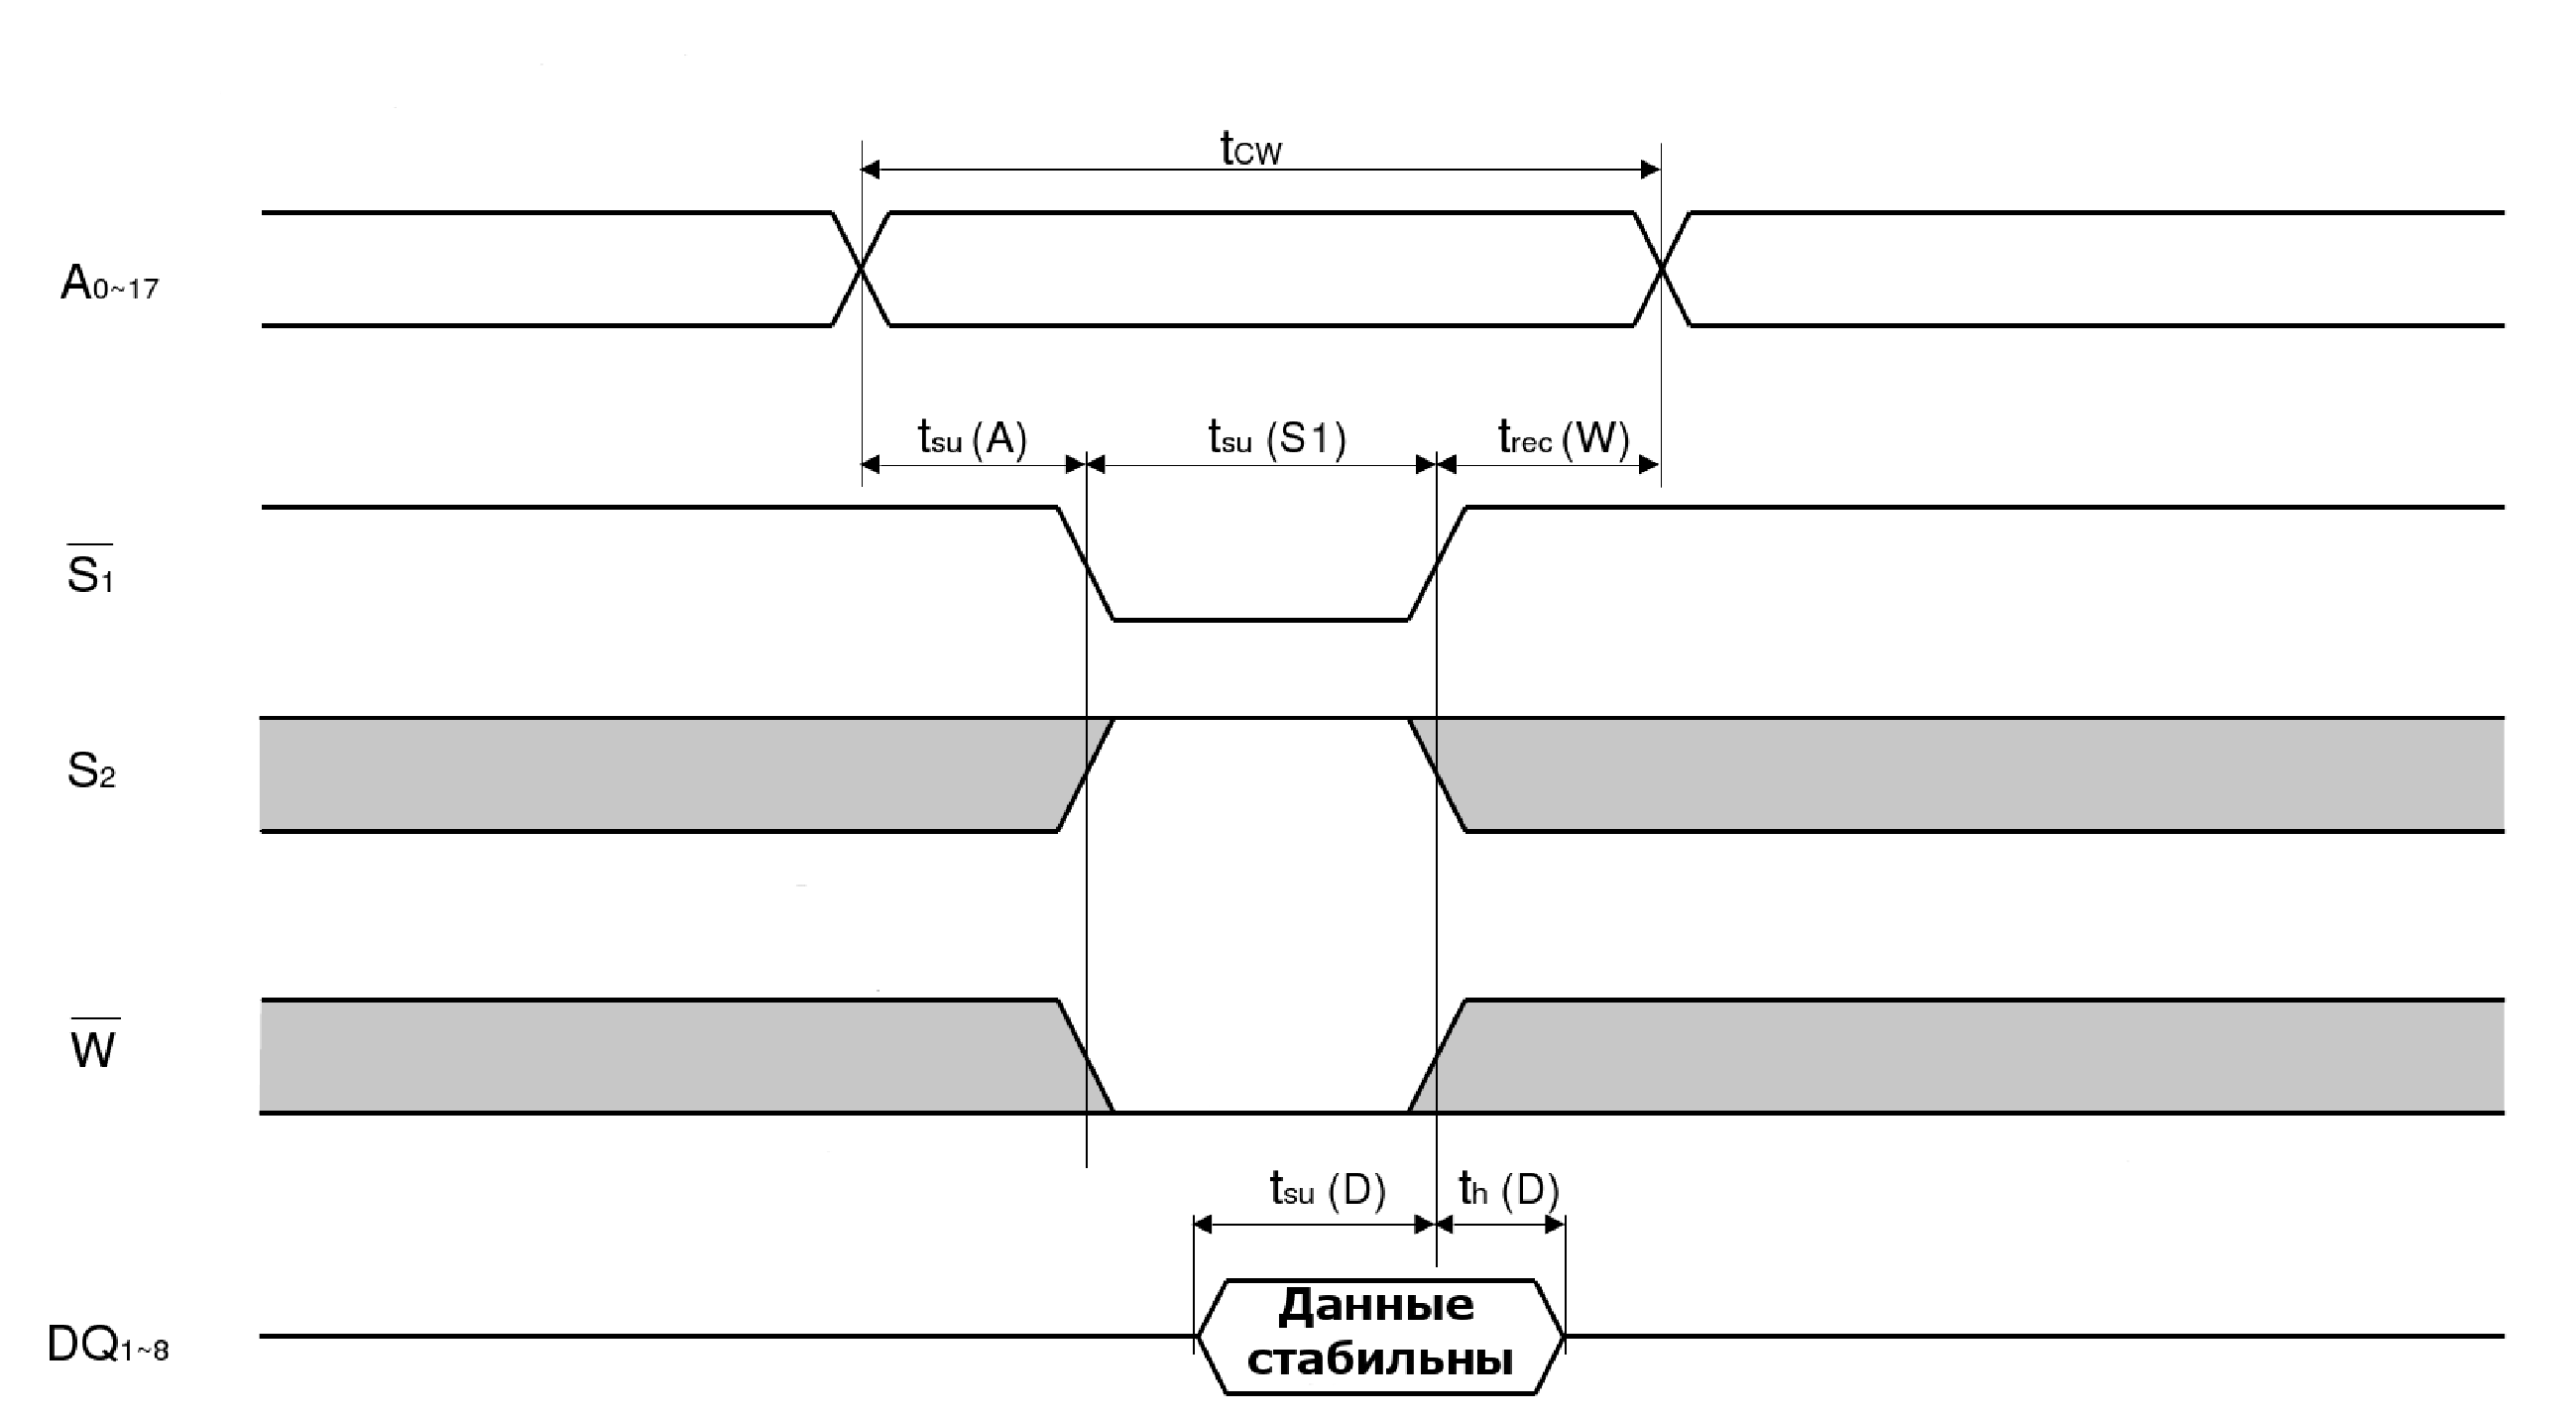
\includegraphics[width=1\linewidth]{./pics/sram_write_cycle.eps} }
\caption{Цикл записи}
\label{pic:sram_write_cycle}
\end{figure}

\begin{table}[H]
\begin{center}
\caption{Цикл операции записи в SRAM}
\label{tab:sram_write_cycle}
\begin{tabular}{|c|c|c|c|}
	\hline
		Название цикла & Обозначение & Время & Единицы \\
	\hline
		${t_{cw}}$ & Время цикла записи & 85 & ns \\
	\hline
		${t_w(W)}$ & Вркмя пульса записи & 60 & ns \\
	\hline
		${t_{su}(A)}$ & Время установки адреса & 0 & ns \\
	\hline
		${t_{su}(A-WH)}$ & Время установки адреса в соотв. с $\bar{E}$ & 70 & ns \\
	\hline
		${t_{su}(S_1)}$ & Время установки Chip Select 1 & 70 & ns \\
	\hline
		${t_{su}(S_2)}$ & Время установки Chip Select 1 & 70 & ns \\
	\hline
		${t_{su}(D)}$ & Время установки данных & 35 & ns \\
	\hline
		${t_{h}(D)}$ & Время удержания данных & 0 & ns \\
	\hline
		${t_{rec}(W)}$ & Время восстановления & 0 & ns \\
	\hline
		${t_{dis}(W)}$ & Время перехода после $\bar{W}$ низкого & 30 & ns \\
	\hline
		${t_{dis}(OE)}$ & Время перехода после $\bar{OE}$ высокого & 30 & ns \\
	\hline
		${t_{en}(W)}$ & Время перехода после $\bar{W}$ высокого & 30 & ns \\
	\hline
		${t_{en}(OE)}$ & Время перехода после $\bar{OE}$ низкого & 30 & ns \\
	\hline
\end{tabular}
\end{center}
\end{table}

Цикл чтения выполняется при высоком уровне сигнала $\bar{W}$ и низком уровне сигнала OE. В то же время сигналы
$\bar{S_1}$ и ${S_2}$ должны находится в активном состоянии. Подробнее последовательность действий отражена на
Рис.~\ref{pic:sram_read_cycle} и Таблице~\ref{tab:sram_read_cycle}.
Техническая реализация рассмотрена в разделе~\ref{sec:sram_controller} \\

\begin{figure}[H]
\center{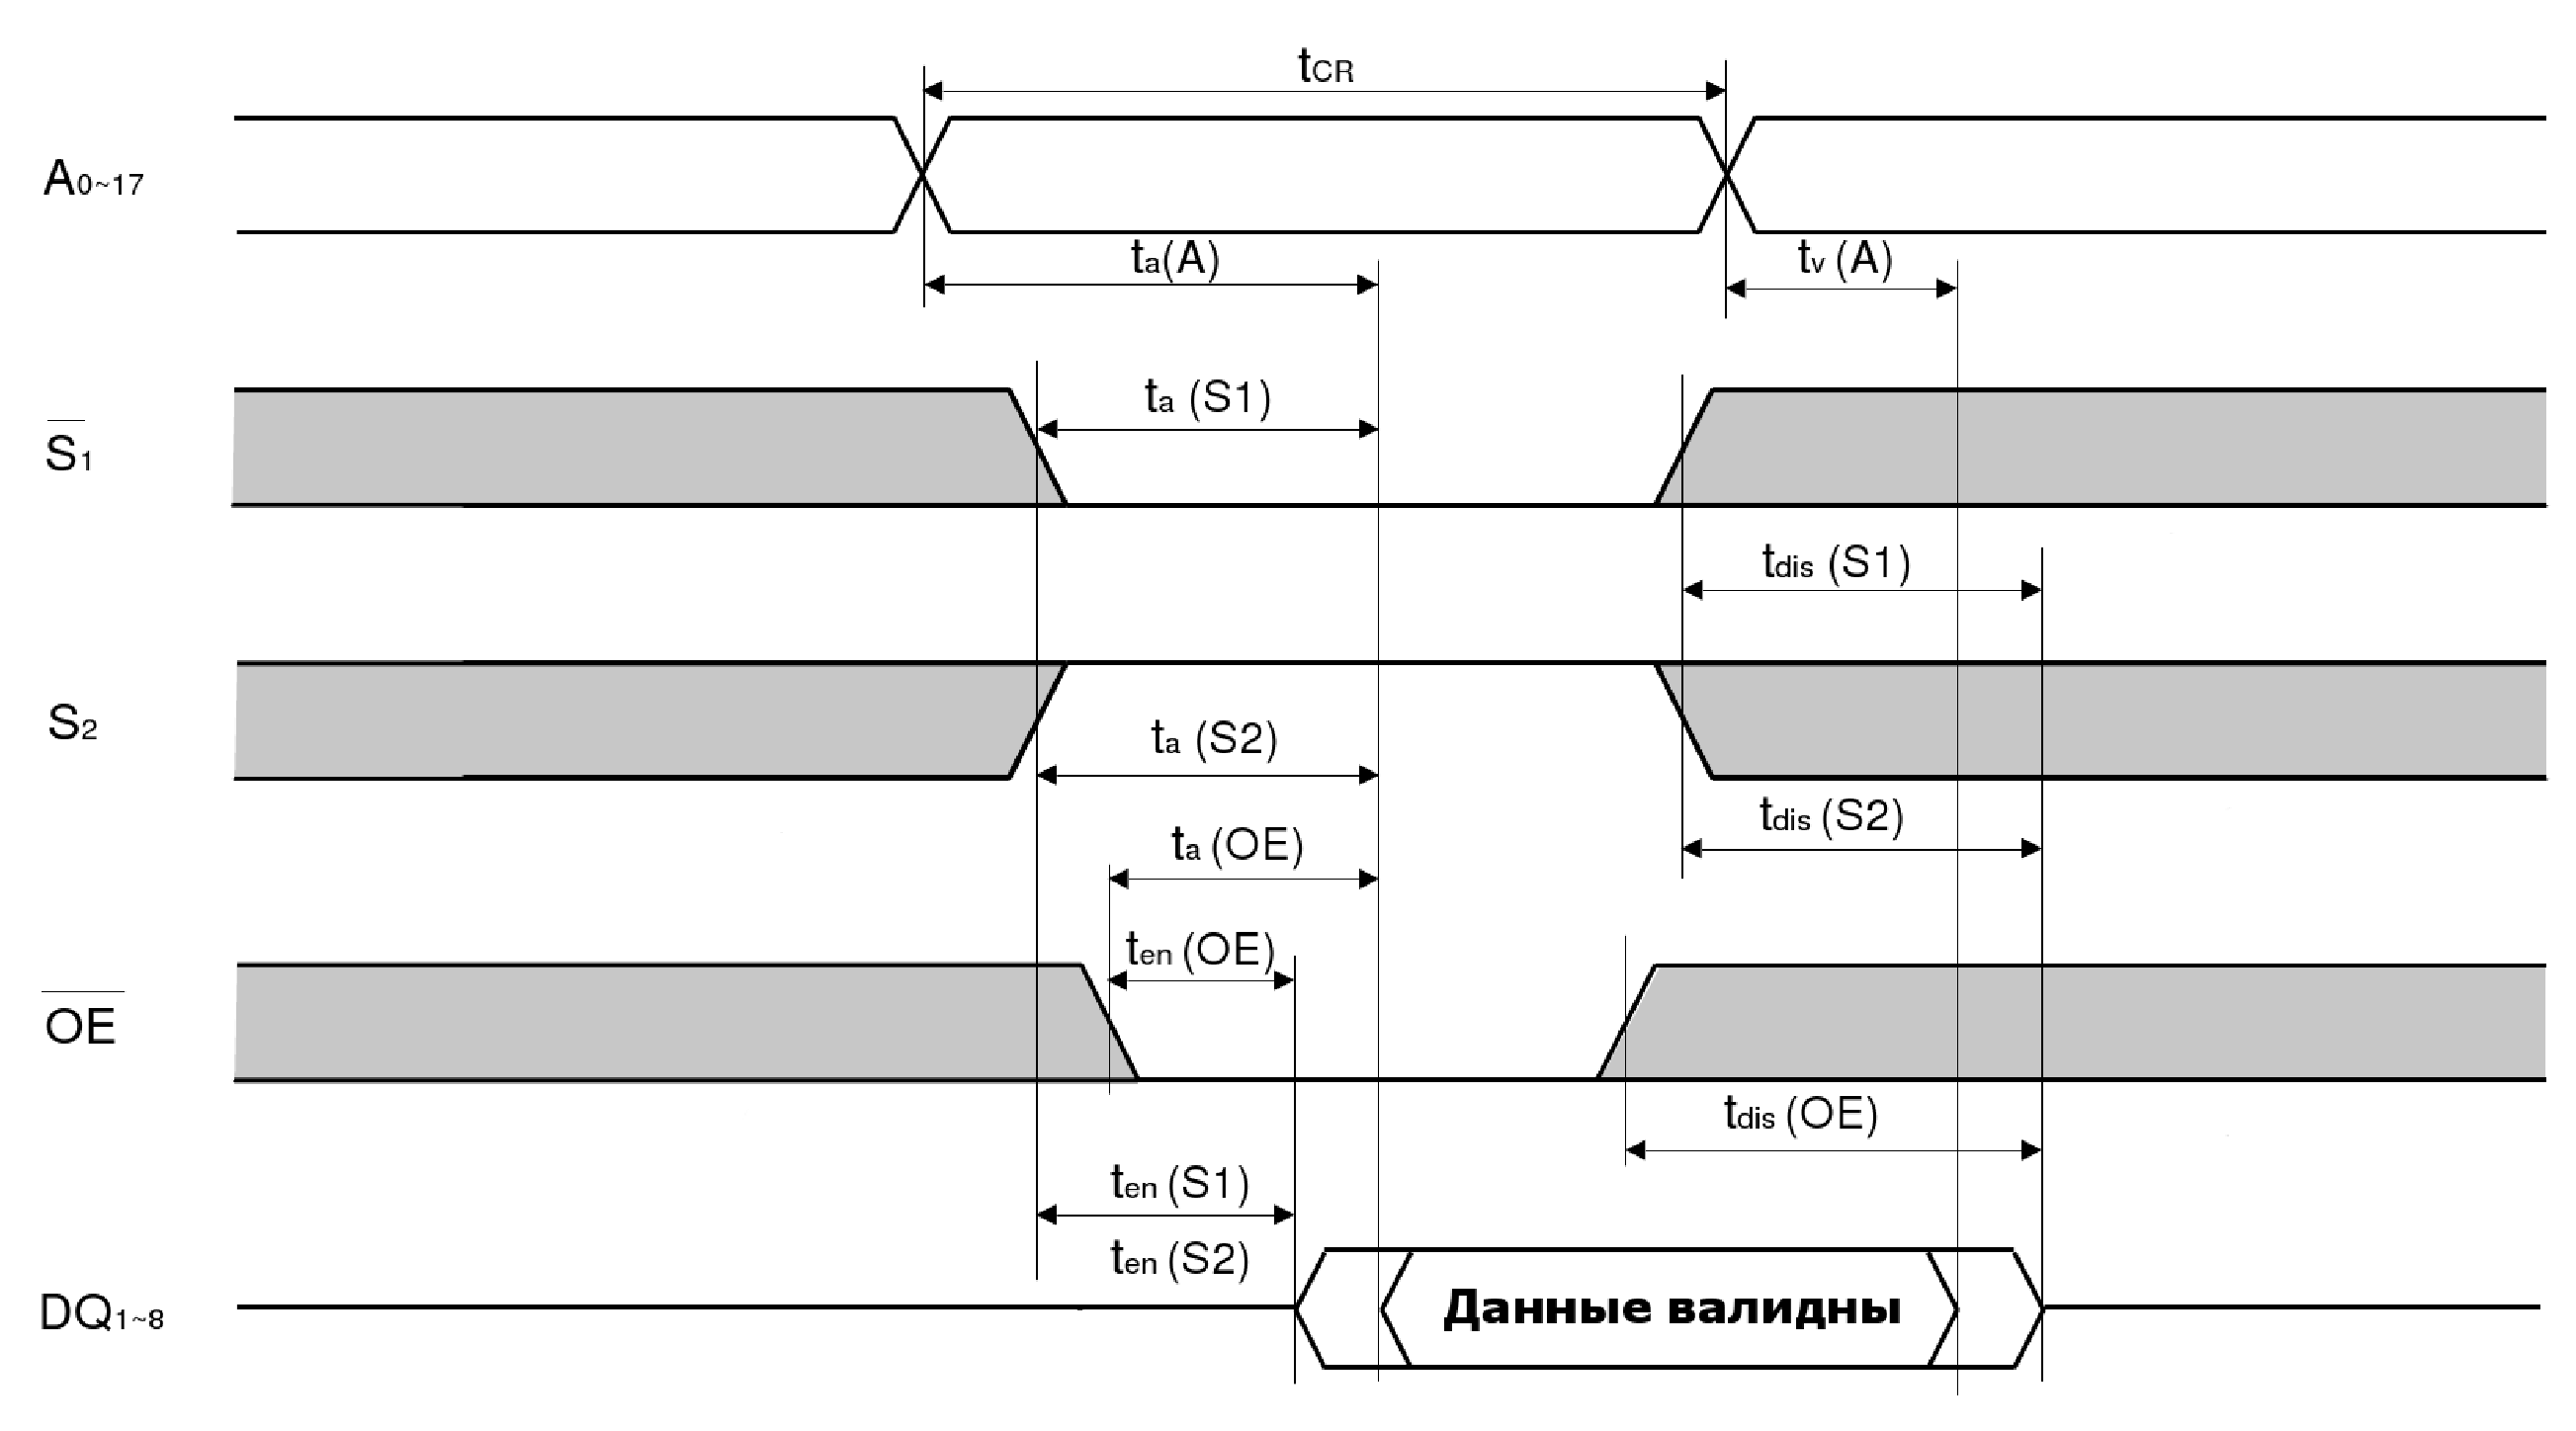
\includegraphics[width=1\linewidth]{./pics/sram_read_cycle.eps}}
\caption{Цикл чтения}
\label{pic:sram_read_cycle}
\end{figure}

\begin{table}[H]
\begin{center}
\caption{Цикл операции чтения из SRAM}
\label{tab:sram_read_cycle}
\begin{tabular}{|c|c|c|c|}
	\hline
		Название цикла & Обозначение & Время & Единицы \\
	\hline
		${t_{cr}(A)}$ & Время цикла чтения & 85 & ns \\
	\hline
		${t_a(A)}$ & Время доступа к адресу & 85 & ns \\
	\hline
		${t_a(S_1)}$ & Chip Select 1 & 85 & ns \\
	\hline
		${t_a(S_1)}$ & Chip Select 2 & 85 & ns \\
	\hline
		${t_a(OE)}$ & Время доступа к активному уровню OE & 45 & ns \\
	\hline
		${t_{dis}(S_1)}$ & Время перехода к низкому уровню & 30 & ns \\
	\hline
		${t_{dis}(S_2)}$ & Время перехода к низкому уровню & 30 & ns \\
	\hline
		${t_{dis}(OE)}$ & Время перехода после $\bar{OE}$ высокого уровня & 30 & ns \\
	\hline
		${t_{en}(S_1)}$ & Переход к активному состоянию для $\bar{S_1}$ & 10 & ns \\
	\hline
		${t_{en}(S_1)}$ & Переход к активному состоянию для ${S_2}$ & 10 & ns \\
	\hline
		${t_{en}(OE)}$ & Переход к активному состоянию для $\bar{OE}$ & 5 & ns \\
	\hline
		${t_{v}(A)}$ & Время валидности данных $\bar{OE}$ & 10 & ns \\
	\hline
\end{tabular}
\end{center}
\end{table}

Полное описание работы данной SRAM-микросхемы памяти приводится в описании на микросхему M5M5V208FP-85 \cite{sram}.

%--------------------------------------------------------------------------------
\subsection{Контроллер последовательного интерфейса для GPS микросхемы MAX2769}
Программирование режимов GPS микросхемы происходит через последовательный порт. Временные критерии и их значения
отражены на рисунке~\ref{pic:gps_serial} и таблице.~\ref{tab:gps_serial} соответственно. Техническая реализация приведена в
разделе \ref{sec:gps_program}.

\begin{figure}[h]
\center{\includegraphics[width=1\linewidth]{./pics/gps_serial_times.eps}}
\caption{Временная диарамма serial-интерфейса GPS}
\label{pic:gps_serial}
\end{figure}

\begin{table}[h]
\caption{Временные требования для serial-интерфейса}
\label{tab:gps_serial}
\begin{tabular}{|c|p{250pt}|c|p{70pt}|}
 \hline  
  Символ & Параметр & Значение & Единица измерения  \\  
 \hline  
  $t_{css}$  & Время между падающим фронтом сигнала $\bar {CS}$ и передним фронтом сигнала SCLK	& 10 & нс  \\  
 \hline  
  $t_{ds}$   & Время установки данных на serial-линию	& 10 & нс \\  
 \hline  
  $t_{dh}$   & Время удержания данных на serial-линии	& 10 & нс \\  
 \hline  
  $t_{ch}$   & Время нахождения Сlock-сигнала serial-интерфейса в состоянии 1 & 25 & нс \\  
 \hline  
  $t_{cl}$   & Время нахождения Сlock-сигнала serial-интерфейса в состоянии 0 & 25 & нс \\  
 \hline  
  $t_{csh}$  & Время между крайним возрастающим фронтом сигнала SCLK и падающим фронтом сигнала $\bar {CS}$ & 10 & нс \\  
 \hline  
  $t_{csw}$  & Время $\bar {CS}$ в активном состоянии    & 1 & такт \\  
 \hline  
\end{tabular}
\end{table}

Значения регистров можно найти в руководстве на микросхему MAX2769 \cite{gps_max}.
\newpage
